% Chapter Template

\chapter{Introduction and Motivation} % Main chapter title

\label{Chapter1} % Change X to a consecutive number; for referencing this chapter elsewhere, use \ref{ChapterX}

%----------------------------------------------------------------------------------------
%	SECTION
%----------------------------------------------------------------------------------------

\section{Introduction}

In many modern-day applications and computer programs, we may encounter frequently a situation where users have to browse or interact with a large set of data or information, however, only focusing only on a certian part of them. In many situations, this part is usually a lot smaller than the original dataset relatively. The most commonly seen scenario would be a \gls{gis} programs on computers, for example an overview + details display shown in \gmref{fig:usgsmap}. These type of applications usually have a zoomable interface to allow users to zoom into a specific region of the original dataset. Also they usually allow users to browse around the dataset from the current focus region and navigate and interact with the whole large dataset with the sense of the ``large picture'' by the mechanism of overview + details techniques.

\begin{figure}[th]
\centering
% 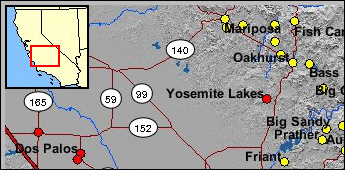
\includegraphics[width=\textwidth,keepaspectratio]{Figures/Chapter1/usgsmap.png}
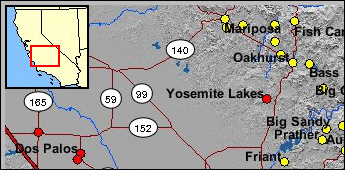
\includegraphics{Figures/Chapter1/usgsmap.png}
\decoRule
\caption[Overview Plus Details On Map]{From \url{http://wildfire.usgs.gov}, an overview of the graphics next to a zoomed ``detail view''.}
\label{fig:usgsmap}
\end{figure}

Other examples besides \gls{gis} include also some image processing, image generation applications such as Photoshop shown in \gmref{fig:ps}, because usually the resolution of the image being processed or generated are larger than the resolution of one single screen monitor. Another interesting example would be in the modern computer gaming industry, that the concept of \emph{Mini-map}s were invented, illustrated in \gmref{fig:minimap}, with the same concepts due to the fact that the virtual world of digital games are mostly a lot larger than how much one single screen can contain.

\begin{figure}[th]
\centering
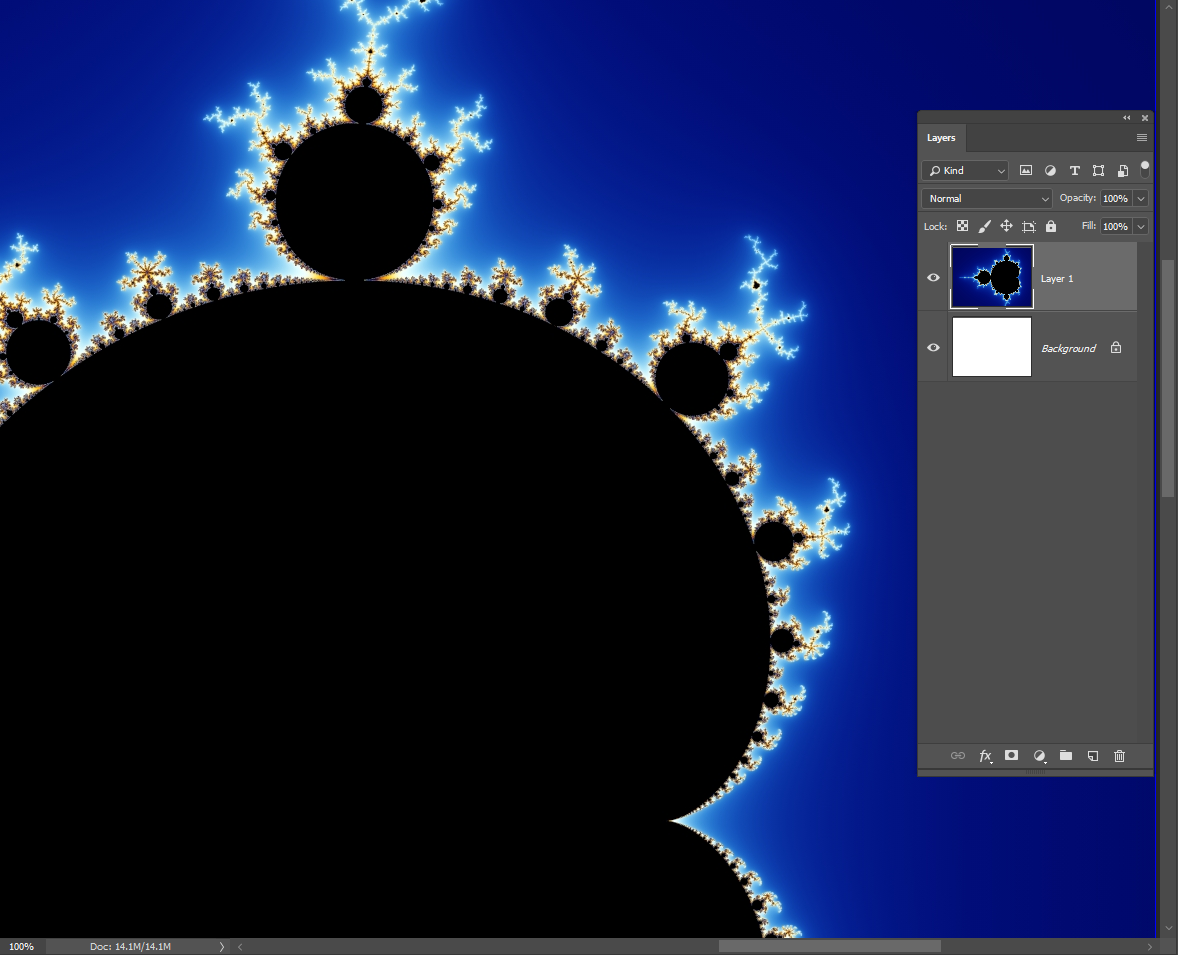
\includegraphics[width=\textwidth,keepaspectratio]{Figures/Chapter1/ps.png}
% 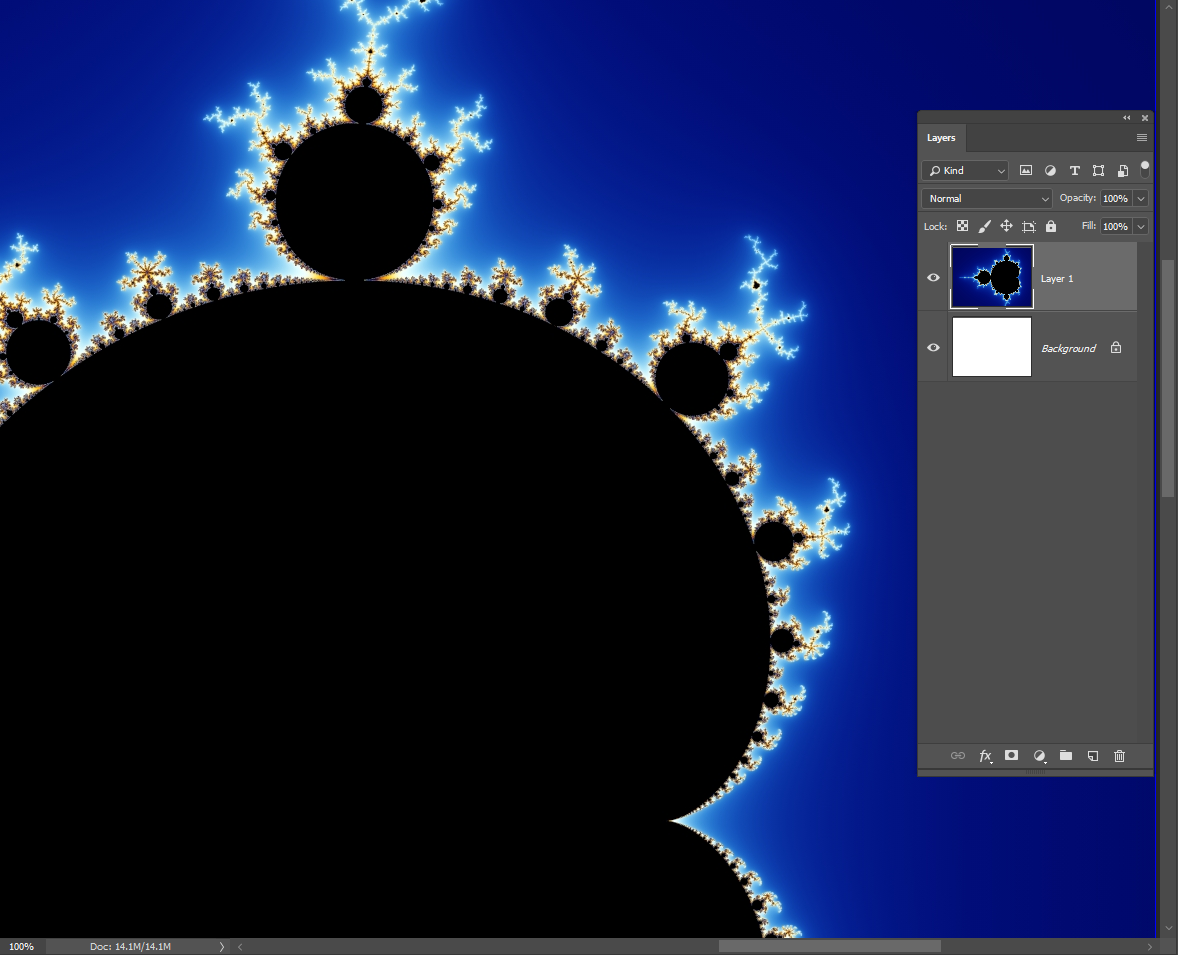
\includegraphics{Figures/Chapter1/ps.png}
\decoRule
\caption[Overview Plus Details In Photoshop]{The basic mechanism in the application Photoshop, layers, offering an overview functionality, with detailed focus area on the main visual area.}
\label{fig:ps}
\end{figure}

\begin{figure}[th]
\centering
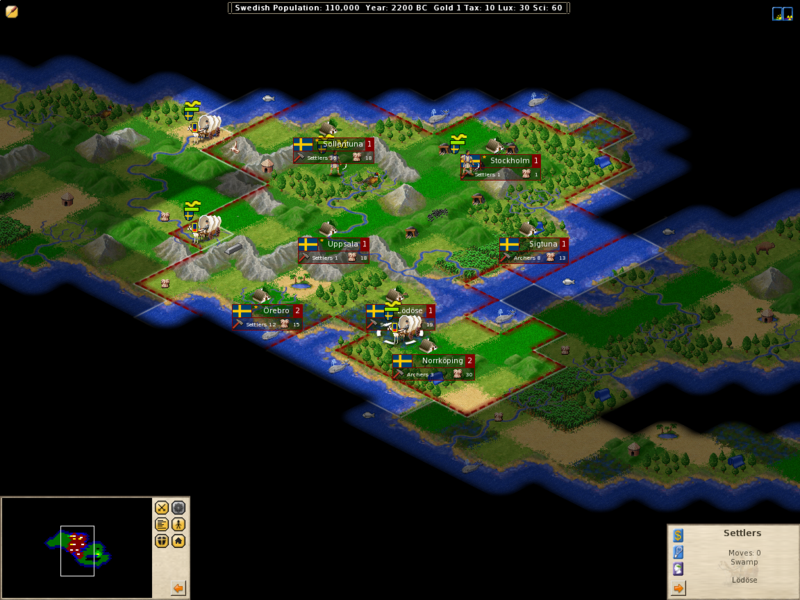
\includegraphics[width=\textwidth,keepaspectratio]{Figures/Chapter1/minimap.png}
% 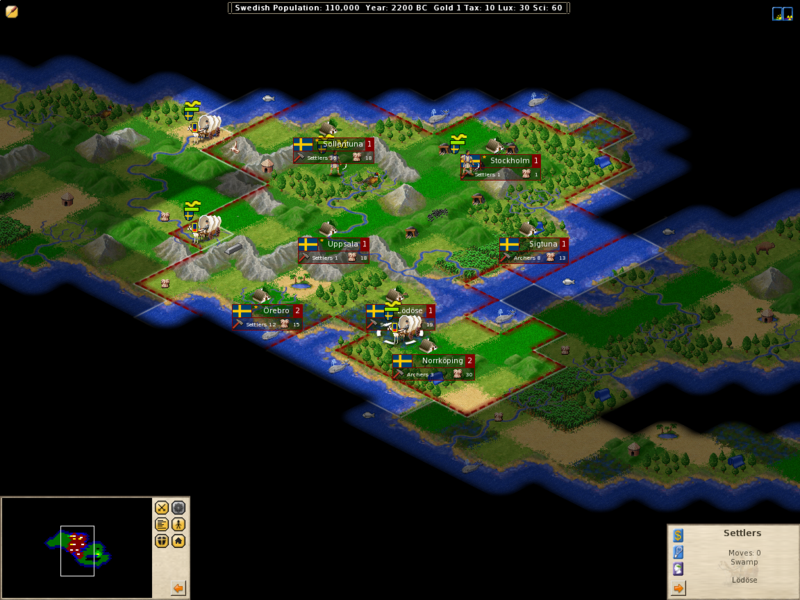
\includegraphics{Figures/Chapter1/minimap.png}
\decoRule
\caption[Overview Plus Details In Computer Games]{The computer game \emph{Freeciv} has a mini-map in the bottom left corner. This is a similar concept as ``Overview + Details''. On this mini-map the white rectangle represents the area of the map currently visible on the main screen. The different colors represent land and ocean and the territories of the different players. The white dots are the position of cities and the blackness are the unexplored areas (the ``fog of war'')\cite{wiki:minimap}.}
\label{fig:minimap}
\end{figure}

Note that the term of \emph{Overview + Details} sometimes are also referred to as \emph{Focus + Context}, \emph{Mini-map} or some other terms, however, they are referring to a similar techniques or concepts. 

%----------------------------------------------------------------------------------------
%	SECTION
%----------------------------------------------------------------------------------------

\section{Motivation For More Complicated Situations}

Most of these techniques and examples above are feasible and can improve how human comprehend the information or datasets is because the whole context area, although larger than how much one screen can hold, comparing to the focus area, is still not so much bigger. If you're looking at a street plan of a city, the focus area can still be visibly represented as a rectangle if the context area is only as large as a city. If you're looking at an image with the resolution of twice as wide and tall as your screen monitor, the focus area still has a quarter of the size of the context area.

However, there are situations when these techniques will not be able to improve our comprehension of the whole dataset in a very good way, that is when the resolution of the original dataset is getting too high and the focus area is zoomed in into an extremely detailed state. That way, the focus region becomes a ``dot'' instead of a region to be represented on the context view, losing its width and height properties and stops giving intuitive information. A simple example is shown in \gmref{fig:becomespoint} indicating that when the resolution of the dataset is extreme, new approaches need to be taken in order to let the users able to ``grab the whole picture''.

\begin{figure}[H]
\centering
% 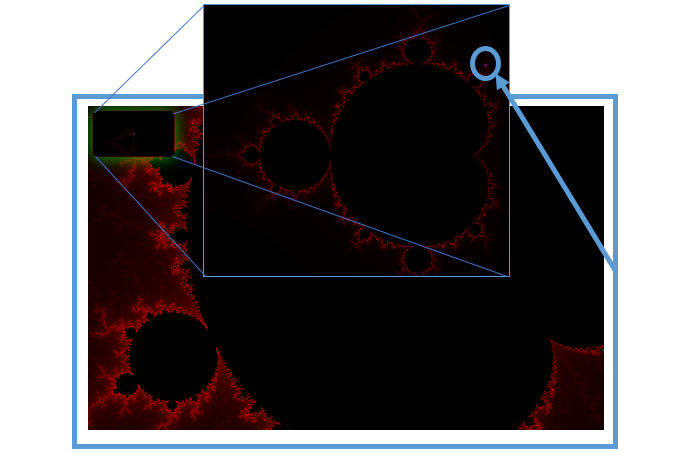
\includegraphics[width=\textwidth,keepaspectratio]{Figures/Chapter1/becomespoint.png}
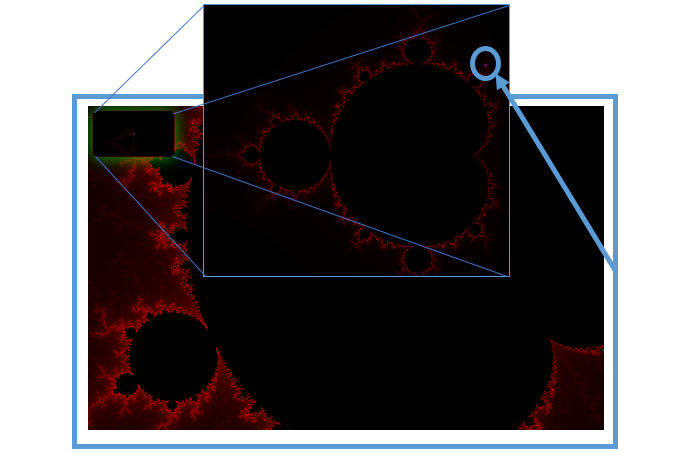
\includegraphics{Figures/Chapter1/becomespoint.png}
\decoRule
\caption[Focus Region Becomes A Dot On Context Region]{Traditional overview + details techniques stop to provide intuitive information on a highly zoomed-in fractal image.}
\label{fig:becomespoint}
\end{figure}

In these situations, a new level of the overview + details techniques is introduced, which is to provide more levels of overviews to the user. Take what's shown in \gmref{fig:zeus} as an example, multiple levels of information of objects are presented as overviews for the users to browse and search. For a similar solution as shown previously in \gmref{fig:becomespoint}, a solution shown in \gmref{fig:multiplelevels} is to give multiple hierarchical overviews to the user to preserve the intuitiveness of the techniques.

\begin{figure}[H]
\centering
% 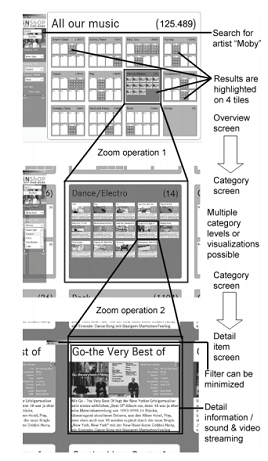
\includegraphics[width=\textwidth,keepaspectratio]{Figures/Chapter1/zeus.png}
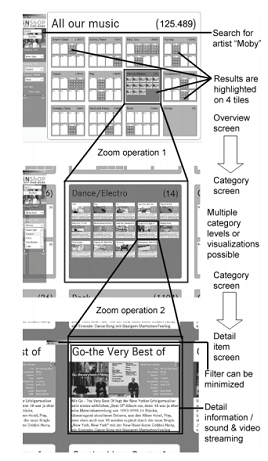
\includegraphics{Figures/Chapter1/zeus.png}
\decoRule
\caption[Multiple Levels of Overview Plus Details]{ZEUS from overview to detail view by zoom in\cite{gundelsweiler2007zeus}.}
\label{fig:zeus}
\end{figure}

\begin{figure}[H]
\centering
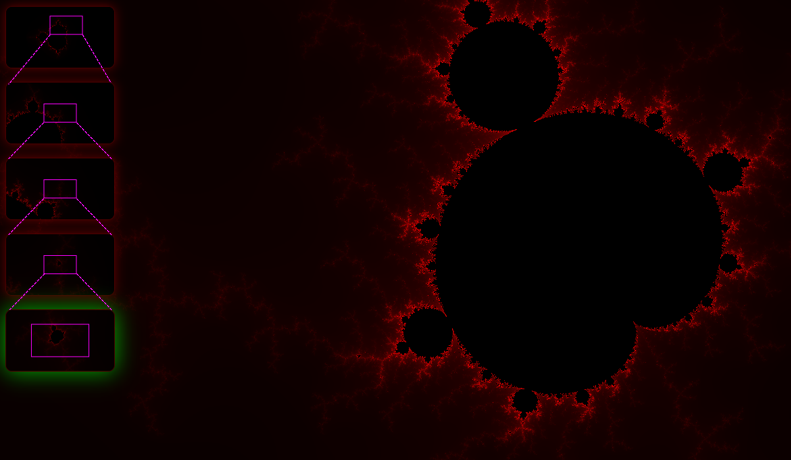
\includegraphics[width=\textwidth,keepaspectratio]{Figures/Chapter1/multiplelevels.png}
% 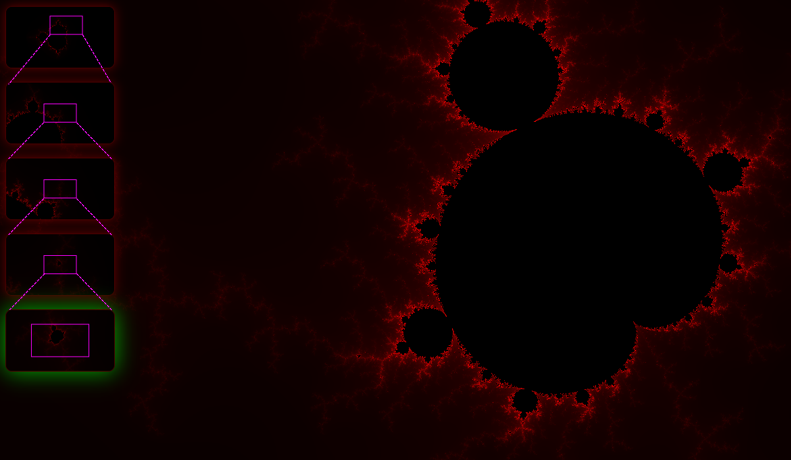
\includegraphics{Figures/Chapter1/multiplelevels.png}
\decoRule
\caption[Zoomed-in Fractal Image]{A graphical representation of Mandelbrot set zoomed in for around $35$ thousand times compared to the original.}
\label{fig:multiplelevels}
\end{figure}

This solution is straightforward, however, we can still raise questions to push the topic into new levels --- what happens when the resolution of the dataset increases even more?

In this case, more overviews need to be added and presented to the users. When more overviews are added providing more \glspl{lod} and contexts and put to the screen, the original problem emerges again --- these overviews are going to occupy a large portion even the entire screen monitor so the most zoomed-in detail area, the most important area of interest, is not going to be easily comprehended or even not able to be seen, as shown in \gmref{fig:occupiesscreen}. 

\begin{figure}[H]
\centering
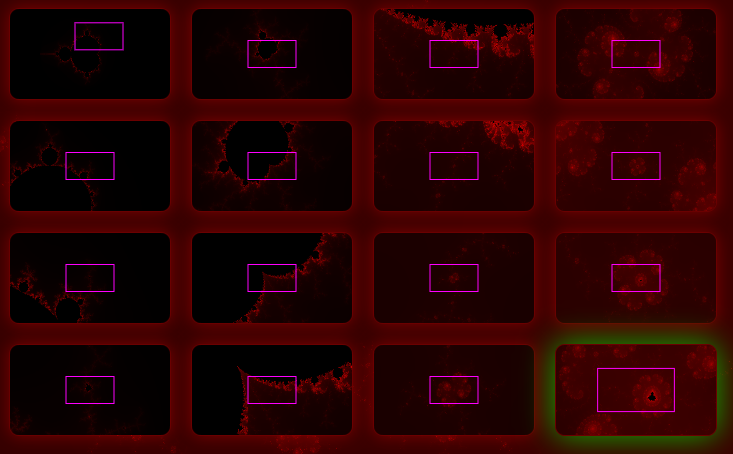
\includegraphics[width=\textwidth,keepaspectratio]{Figures/Chapter1/occupiesscreen.png}
% 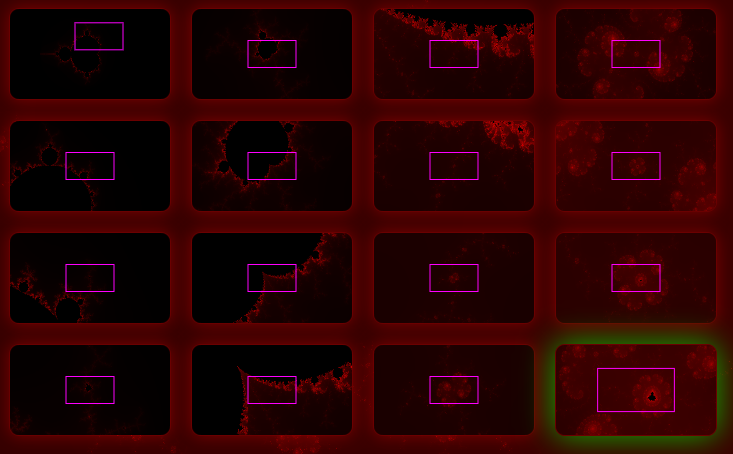
\includegraphics{Figures/Chapter1/occupiesscreen.png}
\decoRule
\caption[Occupied Screen]{Too many overviews occupying entire screen monitor.}
\label{fig:occupiesscreen}
\end{figure}

Therefore, the topic of this thesis is focused on solving this problem, to arrange these overviews in certain ways that they can all provide hierarchies of overviews of information with respect to the original extreme resolution dataset, at the same time, being intuitive enough for human users to understand the \glspl{lod} as well as the most detailed region with the help of all these arrangements.

%----------------------------------------------------------------------------------------
%	SECTION
%----------------------------------------------------------------------------------------

\section{Related Work}

There are many researchers who have already done plenty of work related to the topic of overview + details, focus + context or \gls{lod}.


Single level:

A Review of Overview+Detail, Zooming, and Focus+Context Interfaces\cite{cockburn2009review}

A Review of Focus and Context Interfaces\cite{cockburn2006review}

Navigation Patterns and Usability of Zoomable User Interfaces with and without an Overview\cite{hornbaek2002navigation}

Keeping Things in Context: A Comparative Evaluation of Focus Plus Context Screens, Overviews, and Zooming\cite{baudisch2002keeping}

Focus Plus Context Screens: Combining Display Technology with Visualization Techniques\cite{baudisch2001focus}

Minimap – A Web Page Visualization Method for Mobile Phones\cite{roto2006minimap}

Interacting with Big Interfaces on Small Screens: a Comparison of Fisheye, Zoom, and Panning Techniques\cite{gutwin2004interacting}

The notion of overview in information visualization\cite{hornbaek2011notion}

The Zoom Browser: Showing Simultaneous Detail and Overview in Large Documents\cite{holmquist1998zoom}


Multiple level:

Overview of Multiple Level of Detail Creation\cite{zhigeng1998overview}

Hierarchical geometric models for visible surface algorithms\cite{clark1976hierarchical}

A more flexible image generation environment\cite{crow1982more}

ZEUS–zoomable explorative user interface for searching and object presentation\cite{gundelsweiler2007zeus}